\documentclass[10pt,a4paper]{article}

% Marges du document %
\setlength{\topmargin}{0cm}
\setlength{\headheight}{0.4cm}
\setlength{\headsep}{0.8cm}
\setlength{\footskip}{1cm}
\setlength{\textwidth}{17cm}
\setlength{\textheight}{25cm}
\setlength{\voffset}{-1.5cm}
\setlength{\hoffset}{-0.5cm}
\setlength{\oddsidemargin}{0cm}
\setlength{\evensidemargin}{0cm}

\usepackage{amssymb}
\usepackage{psfrag}
\usepackage[utf8]{inputenc}
\usepackage[francais]{babel}
\usepackage[T1]{fontenc}
\usepackage{amsmath}
\usepackage{amsfonts}
\usepackage{amssymb}
\usepackage{graphicx}
\usepackage{subcaption}
\usepackage{fancyhdr}
\usepackage{multicol}
\usepackage{eurosym} % symbole €
\usepackage{siunitx}
\usepackage{stmaryrd}
\usepackage{bm}

\usepackage{tabu}
\def\€{\euro{}}

\numberwithin{equation}{section}

\newcommand\numberthis{\addtocounter{equation}{1}\tag{\theequation}} 

\usepackage{color} % gestion de différentes couleurs
\definecolor{linkcolor}{rgb}{0,0,0}
\definecolor{linkcolorurl}{rgb}{0,0,1}
\usepackage[ pdftex,colorlinks=true,
pdfstartview=FitV,
linkcolor= linkcolor,
citecolor= linkcolor,
urlcolor= linkcolorurl,
hyperindex=true,
hyperfigures=false]
{hyperref} % fichiers pdf 'intelligents', avec des liens entre les références, etc.

% En-tête et pied de page % 
\pagestyle{fancy}
\fancyhead[L]{\scriptsize \textsc{Titre}} 
\fancyhead[R]{\scriptsize \textsc{VERGNET Hadrien}} 
\fancyfoot[C]{ \thepage}

\author{Vergnet Hadrien}


\begin{document}

%%%%%%%%%%%%%%%%%%%%%%%%%%%%%%%%%%%%%%%%%%%%%%%%%%%%%%%%%%%%%%%%%%%%%%%%%%%%%%%%%%%%%%%%
%%%%%%%%%%%%%%%%%%%%%%%%%%%%%%%%%%%%%%%%%%%%%%%%%%%%%%%%%%%%%%%%%%%%%%%%%%%%%%%%%%%%%%%%
\begin{titlepage}
%%%%%%%%%%%%%%%%%%%%%%%%%%%%%%%%%%%%%%%%%%%%%%%%%%%%%%%%%%%%%%%%%%%%%%%%%%%%%%%%%%%%%%%%
%%%%%%%%%%%%%%%%%%%%%%%%%%%%%%%%%%%%%%%%%%%%%%%%%%%%%%%%%%%%%%%%%%%%%%%%%%%%%%%%%%%%%%%%
\thispagestyle{empty}
\setlength{\parindent}{0pt}


\includegraphics[height=1.9cm]{logo-ens.jpg} \hfill 
\includegraphics[height=2cm]{logo_lyon1.jpg} \hfill 
\includegraphics[height=2cm]{logo_univ_lyon.jpg}



Master Sciences de la matière
\hfill
Projet de Géophysique

\textit{École Normale Supérieure de Lyon}
\hfill
VERGNET Hadrien

\textit{Université Claude Bernard Lyon 1}
\hfill
M2 Physique 2016-2017

\vspace{0.5cm}

\hrulefill
\vspace{-0.6cm}

\hrulefill
\begin{center}\bfseries
\begin{huge}
Étude du chauffage par impact dans un planétésimal
\end{huge}
\Large
\vspace{0.4cm}

Projet réalisé par BUNEL Félix et VERGNET Hadrien
\end{center}
\hrulefill
\vspace{-0.6cm}

\hrulefill

\vspace{0.5cm}

\textbf{Résumé :} 
Nous avons réalisé, dans le cadre du module de Géophysique, un modèle numérique d'un planétésimal afin d'étudier l'importance du chauffage par impact sur sa température, en nous basant sur l'article \textit{Thermal evolution and differentiation of planetesimals and planetary embryos. (2012), Icarus, 217(1), 339-354.} par Šrámek, O., Milelli, L., Ricard, Y., et Labrosse, S. .  Notre étude nous a permis de décomposer les différentes contributions au profil de température dans ce planétésimal afin de mettre en évidence l'influence du chauffage par impact.
\vspace{0.3cm}

\textbf{Mots clefs :} planétésimal, accrétion, chauffage
\vspace{0.3cm}



\tableofcontents

\end{titlepage}


\newpage
\renewcommand\thepage{\arabic{page}}

\setcounter{page}{1}

\section*{Introduction}
\addcontentsline{toc}{section}{Introduction}

Pour remettre dans son contexte le sujet de cette étude, revenons d'abord sur les étapes de la formation de notre système solaire. Nous commencerons avec le gigantesque nuage d'hydrogène et d'hélium qui deviendra notre galaxie; dans ce nuage naissent des premières étoiles qui synthétisent en leur cœur les éléments lourds comme le fer et les dispersent à leur mort. Ce nuage désormais enrichi en éléments lourds se fractionne ensuite en plus petits nuages dont un deviendra notre système solaire. Ce petit nuage s'effondre sur lui-même pour donner naissance à notre Soleil. Autour de ce Soleil il reste encore de la poussière qui va progressivement coalescer pour former des corps de plus en plus volumineux jusqu'à devenir des planétésimaux, qui ne sont autre que des embryons de planètes. Ces planétésimaux vont alors grossir par accrétion gravitationnelle de la matière environnante pour finalement devenir des planètes. Le planétésimal est donc un corps céleste de quelques kilomètres de diamètre se trouvant dans une nébuleuse de poussières composées d'éléments lourds. Une caractéristique importante de ces planétésimaux est que leur champs gravitationnel est suffisamment intense pour attirer les autres planétésimaux et la matière environnante et qu'ils peuvent ainsi croître.

Le but de ce  projet a été d'étudier l'influence du chauffage par impact lors de la formation d'un planétésimal par accrétion. Cette étude s'inscrit dans une problématique plus large d'étude des différents scénarios de formations ayant pu mener à la différenciation du noyau et du manteau de la Terre. En effet la formation d'un noyau liquide est principalement conditionnée par la température atteinte  qui permet ou non la fusion du matériau dans le planétésimal. Ainsi nous avons concentré notre étude sur la résolution numérique de l'équation de diffusion de la chaleur dans un planétésimal qui nous a permis de calculer l'évolution de la température $T$ dans celui-ci :

\begin{equation}
\rho C_p \frac{\partial T(\vec{r},t)}{\partial t} =  k_{T} \nabla T(\vec{r},t)  + P(\vec{r},t)
\end{equation}
Où $\rho$, $C_p$ et $k_{T}$ sont respectivement la masse volumique, la capacité calorifique et la conductivité thermique du matériau et $P$ est un terme qui permet de tenir compte des différentes sources de chaleur dans le modèle.



Pour réaliser cette étude nous avons développé, en \texttt{Python}, trois modèles successifs  de complexité croissante, afin de pouvoir distinguer la contribution de chacun des paramètres que nous avons considérés dans notre modèle final.
% le dernier modèle tenant compte de l'évolution du rayon du planétésimal et des deux sources de chaleurs en jeu, à savoir le chauffage radioactif dû au $^{26}$Al et à l'énergie apportée par les impactants qui déposent à la fois leur énergie cinétique et leur chaleur propre, le seul terme de perte de chaleur étant dû aux dissipations radiatives à la surface du planétésimal.
On détaillera ces trois modèles ainsi que les méthodes numériques utilisées pour résoudre numériquement les équations en jeu.


\section{Description du modèle}

\subsection{Hypothèses de départ}

Le modèle que nous avons étudié est celui d'un planétésimal simplifié. Nous avons en particulier supposé que le problème présentait une symétrie sphérique et qu'il pouvait se réduire à un modèle à une dimension en tenant compte de cette symétrie dans les équations. Nous avons ensuite supposé que le planétésimal était constitué d'un mélange homogène de métal et de silicates dans les proportions 18\% de métal pour 82\% de silicates et que les propriétés de ces matériaux ne dépendaient pas de la température, de la pression, ou de l'état (liquide ou solide) du matériau. Dans le continuité de cette hypothèse d'un mélange homogène, nous n'avons pas tenu compte des phénomènes mécaniques qui conduisent à la séparation des matériaux comme la séparation de phases et la percolation, qui ont lieux lors de la fusion des matériaux. Nous avons toutefois tenu compte de l’énergie libérée ou absorbée lors du changement d'état du métal et des silicates.
Avec ces hypothèses l'équation de diffusion de la chaleur qui décrit l'évolution de notre système devient :

\begin{equation}
\rho C_p \partial_{t} T = \frac{k_{T}}{r^2} \partial_{r} (  {r}^2 \partial_{r} T)  + P
\end{equation}

Où $r$ est la coordonnée radiale dans le planétésimal.

Les sources de chaleur que nous avons considérées dans notre planétésimal sont :
\begin{itemize}
\item la chaleur radioactive produite lors de la décomposition du $^{26}$Al,
\item la chaleur échangée à la surface de l'astre avec la nébuleuse environnante par le rayonnement de corps noir, 
\item et la chaleur apportée par l’accrétion via la température propre de l'objet impactant et l'énergie cinétique qu'il dépose par l'impact.
\end{itemize}


Nous nous sommes aussi posé la question de la température initiale à donner au planétésimal, puisque l'on suppose sa formation instantanée au début de chaque simulation. Nous avons considéré une hypothèse consistant à donner une température équivalente à l'énergie potentielle gravitationnelle qu'il faudrait dissiper pour assembler la masse du planétésimal, qui se calcule en intégrant l'énergie nécessaire pour apporter une particule de masse $dm$ de l'infini à une distance $R$ d'un objet de masse $m$ :
$$ dE = G \frac{m dm}{R}$$ sur tout la masse totale initiale du planétésimal. On trouve ainsi que l'énergie totale apportée est donnée par la formule :
$$ E = \frac{3}{5} \frac{GM^2}{R}$$
Ce qui donne l'expression suivante pour la température initiale :
\begin{equation}
T_0 = T_{neb} + \frac{4\pi}{5}\frac{\rho G}{C_p} R^2
\end{equation}
Où $T_{neb}$ est la température de la nébuleuse, $\rho$ et $C_p$ sont la densité et capacité calorifique moyenne dans le planétésimal, $R$ est le rayon du planétésimal et $G$ la constante de gravitation. Or une application numérique pour le rayon initial  $R_0 = 5$\SI{}{km}, que nous avons considéré, révèle que la contribution de l'énergie gravitationnelle $T_{grav} = 0.02$\SI{}{K} est négligeable devant la température de la nébuleuse $T_{neb} = 300$\SI{}{K}. Ainsi l'hypothèse la plus simple consistant à prendre la température de la nébuleuse comme température initiale est justifiée, et c'est ce que nous avons finalement appliqué. 

Dans tous nos modèles, nous avons utilisé la table suivante de constantes physiques pour les matériaux considérés. Nous avons de plus précisé quelques valeurs moyennes utiles pour simplifier certains calculs du fait de l'hypothèse de mélange homogène métal-silicates dans la proportion 18\%-82\%
Les constantes respectives et moyennes du mélange sont les suivantes :
\tabulinesep=0.3mm
\begin{center}
  \begin{tabu}{ r | c c c l}
    Grandeur & moyenne & métal & silicate & unité\\ \hline
    Densité ($\rho$) & 4028 & 7800 &  3200 & \SI{}{kg.m^{-3}}\\ \hline
    Capacité calorifique ($C_p$) & 939 & 450 & 1200 &  \SI{}{J.K^{-1}.kg^{-1}} \\ \hline
    Conductivité ($k_T$)& 11.48 & 50 & 3 & \SI{}{W.K^{-1}.m^{-1}}  \\ \hline    
    Chaleur latente de fusion & 413 & 250 & 500 & \SI{}{kJ.kg^{-1}}\\ \hline
    Température de fusion & & 1261 & 1408 & \SI{}{K}\\ \hline

  \end{tabu}
\end{center}

Pour la suite on notera $\rho$ une valeur moyenne et $\rho_{materiau}$ la valeur respective d'une grandeur pour l'un des matériaux.
On utilisera aussi les constantes supplémentaires suivantes :

\begin{center}
  \begin{tabu}{ r  c }
    \hline
    Constante de Stephan-Boltzman & \SI{5.67E-8}{W.m^{-2}.K^{-4}}  \\ \hline
    Demi-vie du $^{26}$Al & \SI{0.717}{My}  \\ \hline
    Température de la nébuleuse & \SI{300}{K}  \\ \hline
    Chaleur dégagée initiale du $^{26}$Al & \SI{1.5E-7}{W.kg^{-1}}  \\ \hline
  \end{tabu}
\end{center}


\subsection{Méthodes numériques}

Comme nous l'avons mentionné, nous avons considéré un modèle à une seule dimension radiale en tenant compte de la géométrie du planétésimal dans l'équation étudiée:

\begin{equation}
\rho C_p \partial_{t'} T' = \frac{k_{T} }{r'^2} \partial_{r'} ( {r'}^2 \partial_{r'} T')  + P
\end{equation}



Pour éviter tout souci lié à la représentation numérique des grands nombres que nos équations manipulent, nous avons commencé par ré-exprimer cette équation en unités adimentionnées. Pour cela, nous avons introduit les trois variables adimentionnées suivantes en divisant les variables par les grandeurs caractéristiques du modèle, respectivement le temps de demi-vie du $^{26}$Al, la longueur de diffusion dans le planétésimal sur ce temps et la température de la nébuleuse: 


\begin{equation}
t= \frac{t'}{\tau^{Al}_{1/2}}  \quad \textrm{,} \quad   r = r' \sqrt{\frac{\rho C_p} {k_T \tau^{Al}_{1/2}}} \quad  \textrm{et} \quad T = \frac{T'}{T_{neb}} 
\end{equation}

Nous avons ensuite injecté ces nouvelles variables dans notre équation afin d'obtenir une équation adimentionnée:

\begin{equation}
 \partial_{t} T =  \frac{1}{r^2} \partial_{r} ( {r}^2 \partial_{r} T)  + c_0 P 
\end{equation}

Avec :
\begin{equation}
 c_0 = \frac{\tau_{1/2}}{\rho C_p T_{neb}}
\end{equation}


Nous avons discrétisé l'équation sur un maillage régulier à une dimension à l'aide d'une méthode de différence finie implicite. Nous avons utilisé une discrétisation d'Euler centrée en espace et en temps. Les différentes dérivées présentent dans l'équation devenant :

\begin{align}
\partial_t T &\rightarrow  \frac{T^{t+1}_r - T^{t+1}_r}{\Delta t}\\
\partial_r T &\rightarrow  \frac{T^t_{i+1/2} - T^{t}_{i-1/2}}{\Delta r} \\
\frac{1}{r^2}\partial_r (r^2 \partial_r T ) &\rightarrow \frac{1}{r^2_i \Delta r}\Big [ r^2_{i+1/2}\frac{T^t_{i+1} - T^{t}_{i}}{\Delta r} + r^2_{i-1/2}\frac{T^t_{i-1} - T^{t}_{i}}{\Delta r} \Big]
\end{align}

où $\Delta t$ et $\Delta r$ sont les pas de temps et d'espace choisis et où on utilise la notation $T^{t}_i$ pour désigner $T(t,r_i)$ 

En utilisant cette discrétisation, l'équation adimensionnée se réécrit sous la forme de l'équation matricielle suivante :
\begin{equation}
MT^{t+1} = T^t + c_0 P^{t}
\end{equation}

Avec la matrice 
$
M = \Big [ Id + \frac{\Delta t ~ r^2_{i+1/2}}{r^2_i \Delta r^2} ~ d1 + \frac{\Delta t ~ r^2_{i-1/2}}{r^2_i \Delta r^2} ~ d2  \Big]
$
, où :
\begin{equation}
d1=
\begin{bmatrix}
    2      & -1     & -1        & 0     &\dots      & 0 \\
    0      &  1     & -1        & 0     &           & \vdots  \\
    \vdots & \ddots & \ddots    &\ddots & \ddots    & \vdots \\
    \vdots &        & \ddots    &\ddots & \ddots    & 0 \\
    \vdots &        &           &\ddots & 1         &  -1 \\
    0      & \dots  & \dots     &\dots  & 0         &  0
\end{bmatrix}
d2=
\begin{bmatrix}
     0     & 0      & \dots  & \dots    &\dots      & 0 \\
    -1     & 1      & \ddots &          &           & \vdots  \\
    0      & \ddots & \ddots & \ddots   &           & \vdots \\
    \vdots & \ddots & \ddots & \ddots   & \ddots    & \vdots \\
    \vdots &        & 0      &  -1      &  1        & 0\\
    0      & \dots  & 0      &  -1      & -1        & 2 \\
\end{bmatrix}
\end{equation}

Toutefois avant de résoudre cette équation il faut calculer le terme de production de chaleur P. Ce terme contient :

\begin{equation}
 H = \rho H_0 e^{-ln(2) t} \quad \textrm{la production de chaleur par radioactivité }
\end{equation}

\begin{equation}
 S =\frac{\sigma T_{neb}^4}{\Delta r}( 1 - T^4)  \quad \textrm{le rayonnement de corps noir (à la surface uniquement)}
\end{equation}

\begin{equation}
 \Delta H =  \Delta \phi_{met} H_{fus,met} + \Delta \phi_{sil}  H_{fus,sil} \quad \textrm{la chaleur latente de changement d'état}
\end{equation}

où $\Delta \phi_{met}$ et $\Delta \phi_{met}$ sont les variations des proportions liquide-solide pour le métal et les silicates. Pour calculer $\Delta \phi_{met}$ et $\Delta \phi_{met}$ on procède par une méthode prédicteur-correcteur. On résout une première fois l'équation sans tenir compte de cette chaleur pour calculer une nouvelle température, on compare la température obtenue avec la température de fusion de chaque matériau et on calcule, là où cela s'applique, la chaleur latente de changement d'état. On peut alors résoudre à nouveau l'équation en tenant, cette fois, compte du changement d'état. Pour résoudre toutes ces équations matricielles, nous avons utilisé le module d'algèbre linéaire pour les matrices creuses \texttt{scipy.sparse.linalg} qui est inclus dans la librairie \texttt{scipy}.


\section{Modèles numériques}

\subsection{Modèle 1 : Chaleur latente et régimes de diffusion}

\begin{figure}
\centering
\begin{subfigure}{.49\textwidth}
  \centering
  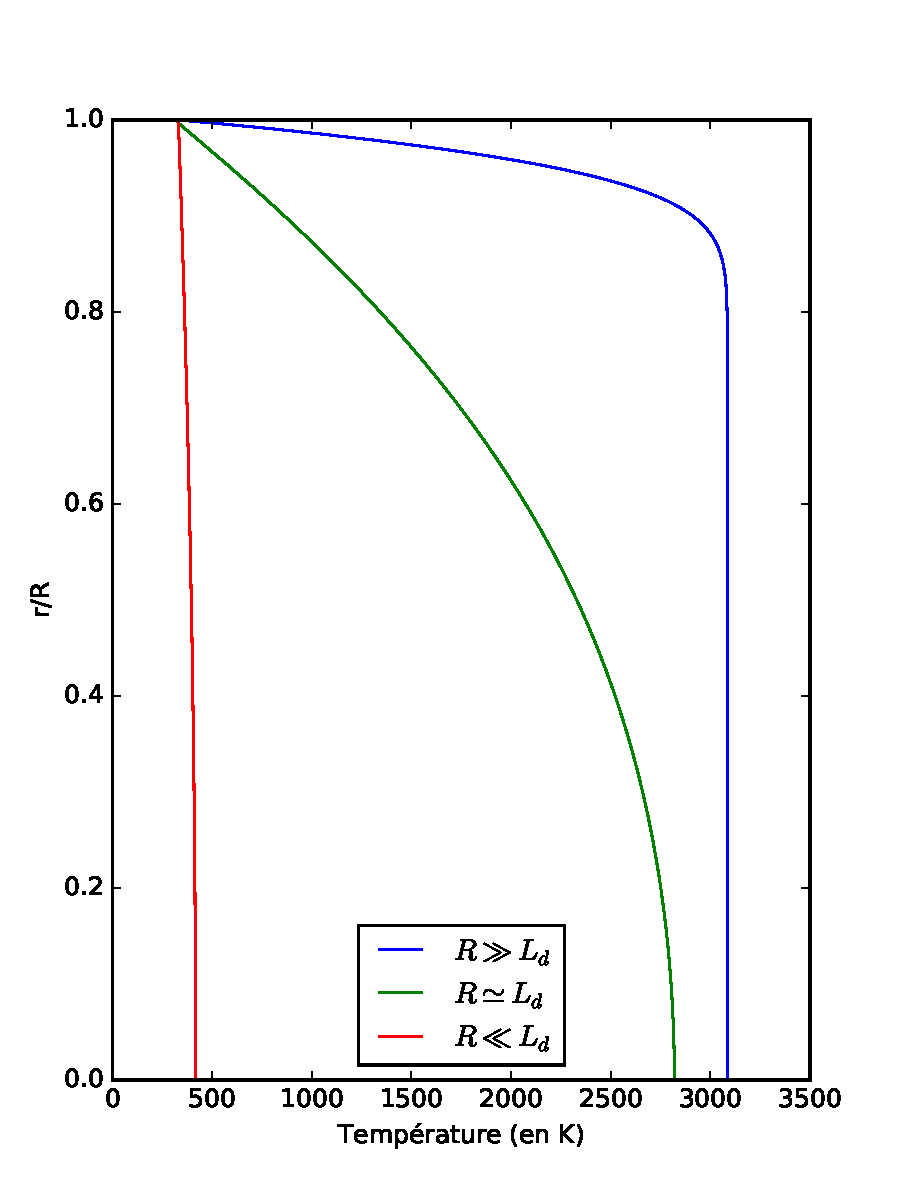
\includegraphics[height=9cm]{./figures/graph_sim1_fig2.pdf}
  \caption{}
  \label{fig1:sub1}
\end{subfigure}
\begin{subfigure}{.5\textwidth}
  \centering
  
  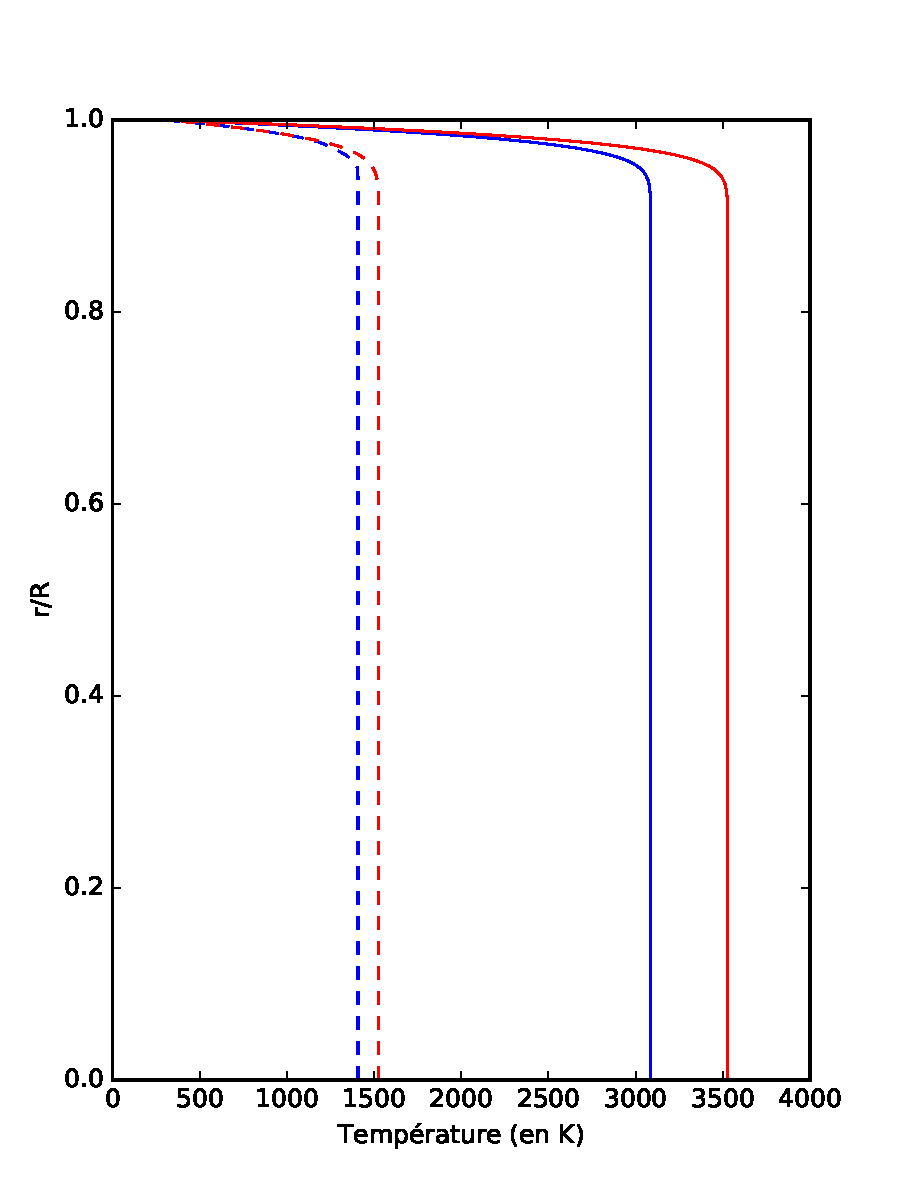
\includegraphics[height=9cm]{./figures/graph_sim1_fig1.pdf}
  \caption{}
  \label{fig1:sub2}
\end{subfigure}%

\caption{On peut voir sur ces figures le profil de température dans une planète après \SI{1}{My} de chauffage par la décomposition radioactive du $^{26}$Al. Sur la figure (a) on peut voir le profil de température après \SI{1}{My} selon le rapport entre le rayon de la planète $R$ et la longueur caractéristique de diffusion $L_d \simeq 10 km $.  Sur la figure (b) on peut voir en trait plein le profil en supposant une origine des temps à \SI{0}{My} et en pointillé une origine des temps à \SI{1}{My}, les courbes bleues tiennent compte de la fusion des matériaux et les courbes rouges n'en tiennent pas compte.}
\label{fig1}
\end{figure}

Dans notre premier modèle nous n'avons pas du tout tenu compte de l'accrétion, nous avons considéré un planétésimal de taille fixée qui n'est chauffé que par la radioactivité du $^{26}$Al et les pertes radiatives. Comme on peut le voir sur la figure \ref{fig1:sub1} on peut observer plusieurs régimes de conduction selon que le rapport entre la taille du planétésimal et la longueur caractéristique de diffusion $L_d$ sur l'échelle de temps considérée qui vaut approximativement \SI{10}{km}. On voit ainsi qu'un planétésimal plus petit que la longueur de diffusion va diffuser très efficacement sa chaleur vers sa surface. Or sa surface est elle-même thermalisée avec la nébuleuse à \SI{300}{K} du fait du transfert radiatif très efficace puisque dépendant de $T^4$. Ainsi la température à l'intérieur du planétésimal n’augmente quasiment pas et vaut \SI{400}{K} au centre. Dans le cas extrême inverse, où le rayon est très grand devant $L_d$, la chaleur diffuse très peu vers la surface pour la majorité de l'épaisseur du planétésimal. Seule une couche d'épaisseur comparable à la longueur de diffusion est affectée par la thermalisation de la surface. La température atteint \SI{3500}{K}, qui correspond à la température atteinte par un système sans perte radiative, sur la majorité de l'épaisseur. Dans le cas intermédiaire la température varie sur l'ensemble de l'épaisseur mais on atteint tout de même \SI{3200}{K} au centre soit \SI{300}{K} de moins que pour le cas précédent.

On peut voir sur la figure \ref{fig1:sub2} que la conséquence  de la prise en compte de la chaleur latente est une différence de température d'environ \SI{440}{K} ce qui correspond exactement à la perte de chaleur attendue lors du changement d'état. Nous avons aussi représenté sur la figure \ref{fig1:sub2} le profil de température final que l'on obtiendrait si le planétésimal s'était formé \SI{1}{My} plus tard et donc si l'abondance du $^{26}$Al était moindre, on voit qu'un retard de \SI{1}{My} réduit considérablement la température finale atteinte qui est environ de \SI{1400}{K}. Ainsi l'abondance initiale du $^{26}$Al radioactif et le délai d'apparition des planétésimaux après la synthèse du $^{26}$Al ont une très grande influence sur le chauffage des planétésimaux.





\subsection{Modèle 2 : Accrétion}

\begin{figure}[h!]
\centering
\begin{subfigure}{.5\textwidth}
  \centering
  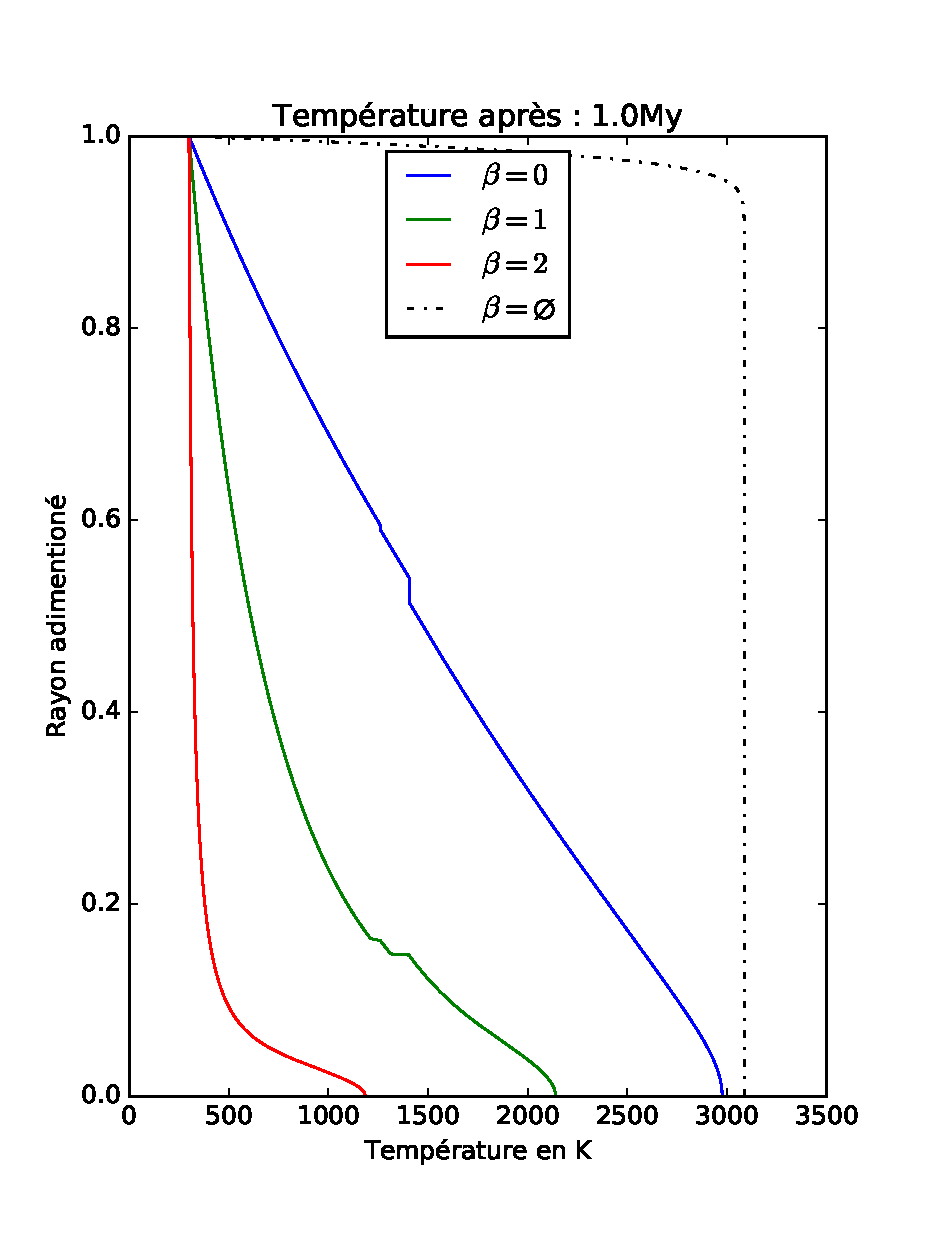
\includegraphics[height=9cm]{./figures/graph_sim2_fig2_1.eps}
  \caption{}
  \label{fig2:1}
\end{subfigure}%
\begin{subfigure}{.5\textwidth}
  \centering
  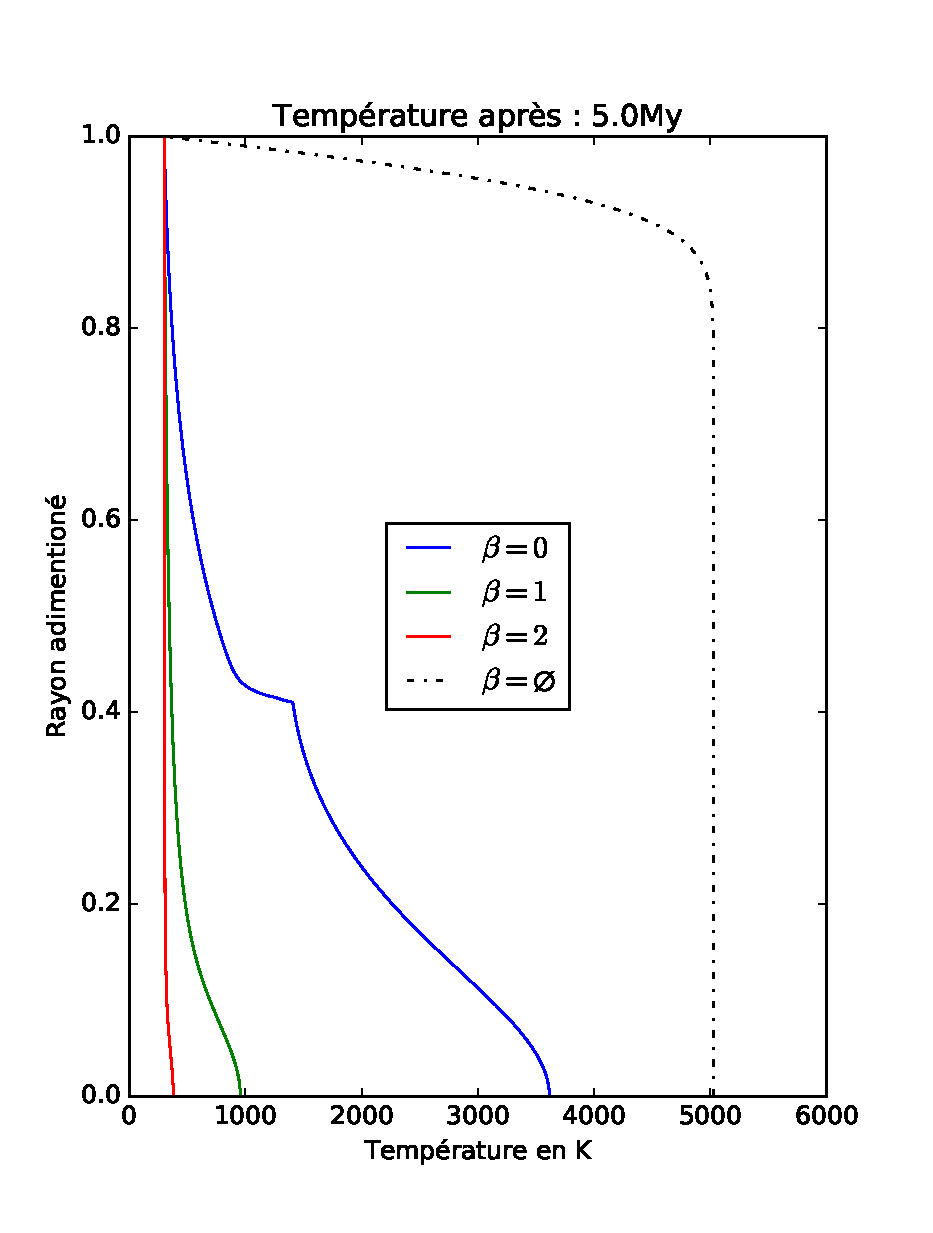
\includegraphics[height=9cm]{./figures/graph_sim2_fig2_2.eps}
  \caption{}
  \label{fig2:2}
\end{subfigure}
\caption{Profil de température dans une planète qui croît par accrétion de \SI{5}{km} à \SI{500}{km} sur une période de \SI{1}{My} sur la figure (a) et de \SI{5}{My} sur la figure (b). Chaque courbe correspond à un taux de croissance différent, les courbes en pointillé  correspondent à un astre dont le rayon est constant à \SI{500}{km} }
\label{fig2}
\end{figure}

Dans ce second modèle, nous avons conservé les même sources de chaleur que pour le modèle précédent en tenant cette fois compte de la variation du rayon provoquée par l'accrétion. Nous avons supposé que la croissance du rayon suivait la loi suivante :

\begin{equation}
\dot{R} \simeq R^\beta  \quad \textrm{avec $\beta$ = 0, 1 ou 2}
\end{equation}

La variation est régulière pour $\beta = 0$ , mais elle est plus explosive pour $\beta = 1$ ou $2$ puisqu'elle accélère avec le temps, on pourra alors distinguer la croissance initiale lente, suivie d'une croissance très rapide vers la fin. 
Nous avons tenu compte de rayon variable dans notre modèle sans changer le maillage mais en ajoutant à l'équation un terme de transport équivalent. L'équation de la chaleur devient :

\begin{equation}
\rho C_p (\partial_{t'} T' - r \frac{\dot{R}}{R}\partial_{r} T')= \frac{1}{r^2} \partial_{r} ( k_{T} \frac{r^2}{R^2} \partial_{r} T')  + P
\end{equation}

Une fois adimentionné et discrétisé, nous avons obtenu une nouvelle équation matricielle que nous avons traité de la même façon que précédemment.
Pour ce modèle, nous avons considéré l'évolution d'un planétésimal partant d'un rayon initial de \SI{5}{km} pour arriver à un rayon final de \SI{500}{km}. 

On peut voir sur la figure \ref{fig2:1} les profils obtenus pour une croissance en \SI{1}{My}. Constate que pour $\beta = 0$ on observe un profil linéaire du centre à la surface du planétésimal, ce qui est cohérent avec la croissance régulière de l'épaisseur du planétésimal. La température au centre est proche de la température maximale. Contrairement au cas $\beta = 1$ et $2$ où la croissance est initialement lente ce qui laisse le planétésimal dans le régime de diffusion efficace pendant une longue période, c'est pourquoi la température au centre reste faible à respectivement \SI{2200}{K} et \SI{1200}{K} pour $\beta = 1$ et $2$. La croissance rapide, qui arrive après cela, ajoute la majorité de l'épaisseur qui n'a pas le temps de chauffer et reste donc proche de \SI{300}{K}.

Dans le cas où la croissance se fait plus lentement, comme on peut le voir sur la figure \ref{fig2:2} on voit que les températures sont largement inférieures à la situation précédente, le planétésimal ne conserve que très peu de sa chaleur puisqu'il a plus de temps pour se thermaliser avec la nébuleuse. On mesure ainsi des températures maximales au centre valant respectivement \SI{3600}{K}, \SI{1000}{K} et \SI{400}{K} pour $\beta = 0$, 1 et 2.


\subsection{Modèle 3 : Chauffage par impact}

\begin{figure}[h!]
\centering
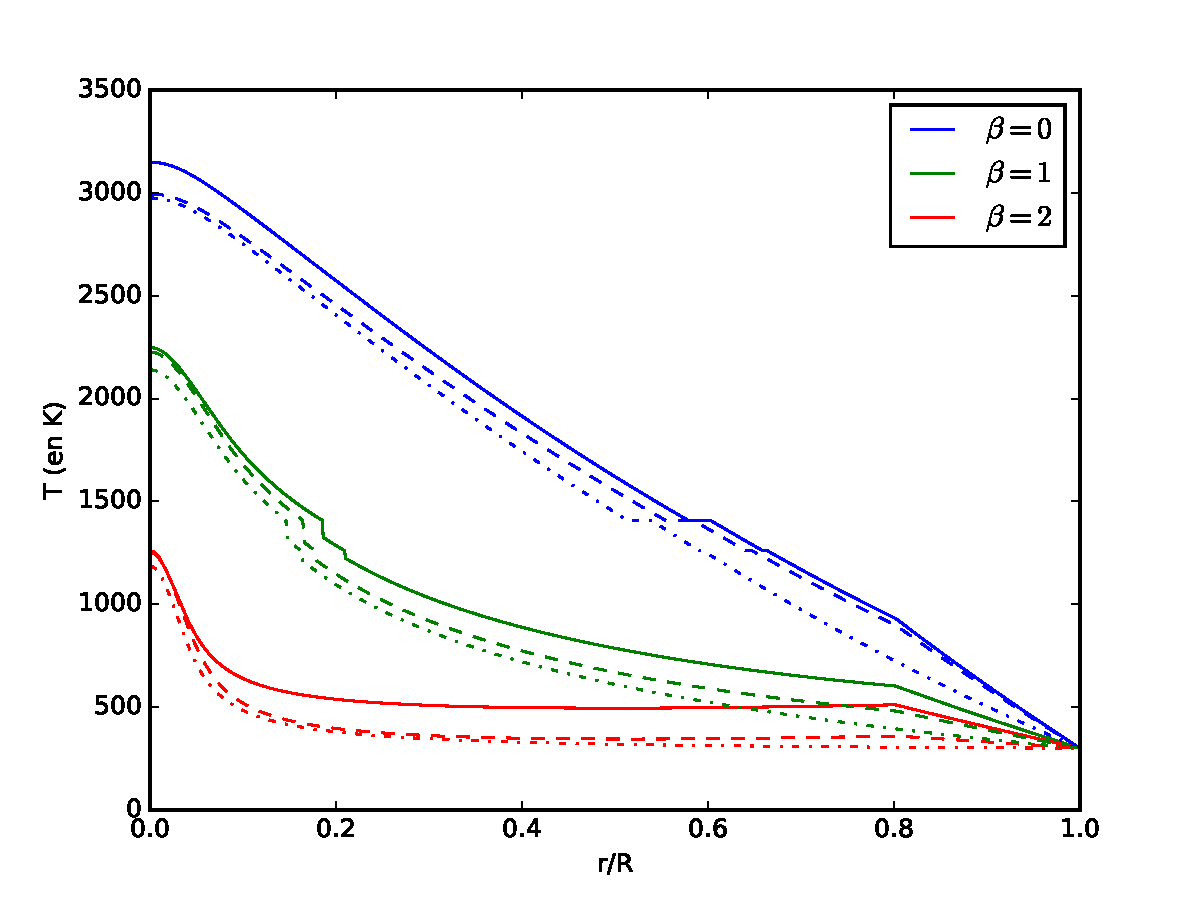
\includegraphics[height=9cm]{./figures/graph_sim3.pdf}
\caption{Profil de température dans une planète qui croît par accrétion de \SI{5}{km} à \SI{500}{km} sur une période de \SI{1}{My}. En traits pleins et en tirets sont tracés les résultats avec chauffage par impact. Les courbes en traits pleins correspondent à un chauffage par impact avec des impacts de température fixe à \SI{1000}{K} et les courbes en tirets correspondent à un chauffage avec des impactants dont la température est calculée via le modèle précédent. En traits pointillés sont rappelés les résultats du modèle précédent sans chauffage par impact.}
\label{fig3}
\end{figure}

Pour notre troisième et dernier modèle, nous avons repris le modèle précédent en ajoutant cette fois l'apport de chaleur des impacts. Cet apport se fait sous deux formes : via la chaleur propre de l'objet impactant et via l'énergie cinétique qu'il dépose lors de l'impact. Toutefois cette énergie est déposée à la surface du planétésimal; or comme on a pu le constater grâce aux modèles précédents, les échanges radiatifs à la surface sont très efficaces, ainsi sur la totalité de l'énergie apportée par l'impact, seule une portion est effectivement déposée dans les couches supérieures du planétésimal, le reste étant immédiatement rayonné vers la nébuleuse. L'article sur le quel nous nous sommes basés proposait une proportion d'énergie conservée comprise entre 20\% et 40\% cette part d'énergie étant déposée sur une épaisseur $R/5$ qui correspond au rayon moyen du planétésimal impactant.
Nous avons considéré deux hypothèses sur la températures des impactants, la première est de supposer leur température fixe égale à \SI{1000}{K}, et la seconde est de supposer que les impactants sont des planétésimaux qui suivent la même évolution que le planétésimal que nous modélisons. Nous avons ainsi calculé la température moyenne en fonction du temps pour des planétésimaux impactants de rayon $R(t)/5$ où $R(t)$ est le rayon du planétésimal que l'on étudie.

On peut constater sur la figure \ref{fig3} que le chauffage par impact avec une température des impactants fixée à \SI{1000}{K} est responsable d'une augmentation de la température quasiment uniforme sur l'ensemble de l'épaisseur du planétésimal d'environ 100 à 200K. 

Quand on considère l'évolution de la température des planétésimaux impactants on trouve un chauffage moindre. Pour $beta = 0$ le chauffage est de quelques dizaines de kelvins au centre et il croit jusqu'à \SI{200}{K} proche de la surface. Pour $beta = 1$ et 2 le chauffage est plus uniforme sur l'épaisseur du planétésimal et vaut environ \SI{100}{K} pour $beta = 1$ et \SI{50}{K} pour $beta = 2$.

On constate ainsi que la contribution du chauffage par impact au profil de température du planétésimal est faible en comparaison à l'influence du chauffage radioactif et de la croissance causée par ces mêmes impacts dans les cas $\beta=0$ et 1. Mais que pour $\beta = 2$ l’augmentation de \SI{200}{K} grâce aux impactants à \SI{1000}{K} est très significative puisqu'on a observé, dans le modèle précédant, que la majorité de l'épaisseur était thermalisé avec la nébuleuse à \SI{300}{K} ou autrement dit totalement froide.

On constate finalement que l'augmentation de température due au chauffage par impact n'est pas ici suffisante pour permettre un noyau fondu la où les autres sources de chaleur ne le permettaient pas déjà.


\section*{Conclusion}
\addcontentsline{toc}{section}{Conclusion}

Avec les trois modèles que nous avons étudiés, nous avons pu constater les contributions de différents paramètres importants sur le profil de température final dans le planétésimal et sur la possibilité ou non de former un noyau fondu. Ainsi nous avons constaté que pour un planétésimal qui croît de \SI{5}{km} à \SI{500}{km} en \SI{1}{My}, le chauffage par impact est responsable d'une élévation de la température de 100 à 200 K uniformément sur la totalité de l'épaisseur du planétésimal. Mais nous avons observé que cette contribution est moins critique que celle du taux de croissance $\beta$ qui conditionne de façon nettement plus importante l'apparition d'un noyau fondu, on avait en effet constaté que pour $\beta = 0$ ou 1 on pouvait observer de la fusion alors que $\beta=2$ la température au centre restait trop faible.
On peut toutefois nuancer ces observations en remarquant qu'à l'instar du calcul que nous avons effectué pour estimer la température initiale du planétésimal, l'énergie déposée par l'impact est proportionnelle au carré du rayon du planétésimal ainsi la contribution du chauffage par impact va dominer pour des planétésimaux plus grands.

\end{document}
